\chapter{规范场、相互作用尺度与带电弱流}

量子电动力学与量子色动力学在实验室中看起来非常不同，但二者都是规范理论。事实上，标准模型中几乎每一种相互作用都是以这种方式组织起来的。\emph{规范}一词具有更深的含义，涉及局域对称性，但我们可以暂且推迟那套机制。眼下我们需要一个最低限度的物理描述：规范理论包含类麦克斯韦场、守恒源、对称变换、规范玻色子，以及发射和吸收这些玻色子的规则。

\section{作为原型的麦克斯韦理论}

\subsection{场与势}

电磁场有六个分量：三个电场分量和三个磁场分量。同样的信息可以（带有一定冗余地）编码在一个四维矢势中
\begin{equation}
A_\mu=(A_0,\boldsymbol A),
\end{equation}
其中\(A_0\)是静电势，\(\boldsymbol A\)是空间矢势。在静电极限下，电场由空间梯度得到，
\begin{equation}
\boldsymbol E=-\boldsymbol\nabla A_0,
\qquad
\boldsymbol F=q\boldsymbol E,
\end{equation}
而磁场为
\begin{equation}
\boldsymbol B=\boldsymbol\nabla\times\boldsymbol A.
\end{equation}
第一个方程中的符号取决于势的标准定义；课堂讨论主要关注的是场是势的导数这一事实。
\editorialnote{对于含时场，完整关系是
\(\boldsymbol E=-\boldsymbol\nabla A_0-\partial_t\boldsymbol A\)。本讲在此有意在较简单的静电层面上展开。}

\begin{figure}[htbp]
\centering
\includegraphics[width=0.62\textwidth]{lecture_05_figure_02.png}
\caption{电磁四维势及其与场的导数关系。}
\lectureframe{00:03:33}
\end{figure}

因此电动力学允许两种等价的描述：一种用\(\boldsymbol E\)和\(\boldsymbol B\)，另一种用\(A_\mu\)。后者只显示四个分量，因为不同的势可以描述相同的物理场。这种冗余正是“规范”一词背后的第一个线索，不过我们暂时还不会正式使用它。

\subsection{波与偏振}

麦克斯韦方程支持波。取一个沿单位矢量\(\hat{\boldsymbol k}\)传播的平面波。在每一点，电场和磁场都是横向的：
\begin{equation}
\boldsymbol E\cdot\hat{\boldsymbol k}=0,
\qquad
\boldsymbol B\cdot\hat{\boldsymbol k}=0,
\qquad
\boldsymbol E\cdot\boldsymbol B=0.
\end{equation}
在\(c=1\)的单位制下，它们的大小相等，
\begin{equation}
|\boldsymbol E|=|\boldsymbol B|.
\end{equation}
对于线偏振波，\(\boldsymbol E\)的方向指定了偏振。整个图样以光速传播。

量子化改变了语言，但没有改变偏振结构。电磁波的量子是光子。把光子画成一个点在所难免会误导人，但可以方便地想象这个点携带一个记录其偏振的小横向指针。四分之一波片或其他光学元件可以旋转该偏振。静态库仑场同样可以（只是粗略地）被想象为来自光子的反复发射和吸收。

\subsection{源、通量与守恒}

电磁波可以在真空中传播，但场也有源：电荷和电流。一个正点电荷产生一个向外的径向电场，正比于\(1/r^2\)。穿过围绕该电荷的任意球面的场线数目与该球面的半径无关。用数学表示，
\begin{equation}
\oint_{S^2}\boldsymbol E\cdot d\boldsymbol S
=\frac{Q_{\mathrm{enc}}}{\epsilon_0},
\label{eq:l5-gauss}
\end{equation}
在SI单位制下。

这不仅仅是一种计算场的便利方法。电场线只能终止于电荷。如果一个孤立电荷简单地消失了，它的场要么必须同时在所有地方消失，违反因果性，要么一个缺失场的前沿必须向外传播，而场线终止于空无一物的空间。两者都不被允许。因此，通量的几何结构使电荷守恒成为自然之事：电荷可以移动，相反电荷可以湮灭，但净电荷不能在没有补偿电流的情况下局域地消失。

相应的局域表述是连续性方程
\begin{equation}
\partial_t\rho+\boldsymbol\nabla\cdot\boldsymbol J=0.
\label{eq:l5-continuity}
\end{equation}
\editorialnote{方程~\eqref{eq:l5-continuity}是课堂上以口头方式展开的因果通量论证的标准局域数学形式。}

\subsection{规范理论的一个实用定义}

现在我们可以陈述这一操作模式了。一个规范理论具有：
\begin{itemize}
\item 类电场与类磁场；
\item 当相互作用足够弱时类似于光波的波；
\item 类似于电荷的源；
\item 将通量与这些源联系起来的Gauss定律；
\item 一条守恒定律以及与之相关的对称性；
\item 场的量子，称为规范玻色子；以及
\item 控制发射与吸收的耦合常数。
\end{itemize}
源不必是电荷。作为一个刻意选取的非物理例子，设想将重子数规范化。质子和中子都具有重子数\(+1\)，因此它们会通过一种新的类Coulomb力相互排斥；而一个质子与一个反质子则会相互吸引。这样的理论在数学上是可以想象的，但自然界并未提供任何观测到的、与重子数耦合的长程规范场。守恒本身并不保证存在规范力。

电荷确实伴随着一种对称性。对于一个带电物质场，
\begin{equation}
\psi(x)\longmapsto e^{i\theta}\psi(x).
\label{eq:l5-u1}
\end{equation}
相位对称性与电荷守恒是同一结构的两个方面。稍后我们可以让\(\theta\)依赖于时空，并看出为什么需要势\(A_\mu\)。这里，整体变换已足以确定守恒电荷。

\section{作为非Abel例子的QCD}

\subsection{三重态、反三重态与胶子矩阵}

在量子色动力学中，一个夸克场带有一个色指标\(i\in\{r,g,b\}\)，并在\(SU(3)\)的基础表示下变换：
\begin{equation}
q'_i=U_{ij}q_j,
\qquad
U^\dagger U=\boldsymbol 1,
\qquad
\det U=1.
\label{eq:l5-q-transform}
\end{equation}
这是三维复色空间中的旋转，而不是普通位置空间中的旋转。这个三分量表示也称为定义表示。

反粒子场由复共轭变量表示。对式~\eqref{eq:l5-q-transform}取复共轭得到
\begin{equation}
q_i^{\prime *}=U_{ij}^*q_j^*.
\label{eq:l5-antiquark-transform}
\end{equation}
因此夸克按\(\boldsymbol 3\)变换，而反夸克按\(\bar{\boldsymbol 3}\)变换。

\begin{figure}[htbp]
\centering
\includegraphics[width=0.62\textwidth]{lecture_05_figure_03.png}
\caption{基础变换及其复共轭反三重态变换。}
\lectureframe{00:18:47}
\end{figure}

\begin{classroomqa}
\audiencequestion{\(U\)矩阵有多少个--七个、八个还是九个？
\lecturetimestamp{00:19:37}}
\lecturerresponse{群元素\(U\)有无限多个。这里所数的有限数目是独立生成元的个数，对于\(SU(3)\)来说是八个。一个一般的\(3\times3\)矩阵有九个矩阵位置，但特殊幺正性留下八个连续方向。}
\end{classroomqa}

胶子场可以写成一个无迹矩阵\(A_{ij}\)。一个指标像夸克那样变换，另一个像反夸克那样变换，因此它的色结构是
\begin{equation}
\boldsymbol 3\otimes\bar{\boldsymbol 3}
=\boldsymbol 1\oplus\boldsymbol 8.
\end{equation}
QCD保留无迹八重态，
\begin{equation}
A_{ii}=\operatorname{tr}A=0,
\end{equation}
并舍弃单态。这就是为什么QCD有八个胶子而不是九个。更一般地，\(SU(N)\)有
\begin{equation}
N^2-1
\end{equation}
个生成元，以及同样数目的规范玻色子场。

光子在电\(U(1)\)下是中性的：旋转电子的相位并不会把光子旋转成不同的光子。胶子则不同。一个胶子带有一个色和一个反色，因此它在伴随表示下变换。例如，一个红--反蓝组合并不是色单态，尽管它包含一个色和一个反色。

\subsection{指标流动与自相互作用}

通过追踪指标可以读出相互作用规则。概略地说，一个色为\(i\)的夸克可以变成一个色为\(j\)的夸克，同时发射一个携带相应色流的胶子：
\begin{equation}
q_i\longrightarrow q_j+A_{ij}.
\label{eq:l5-quark-gluon-vertex}
\end{equation}
\(i\)和\(j\)的精确位置取决于箭头约定；不变的内容是，进入顶点的每一个指标都必须通过另一条线继续下去。没有色指标会丢失。

这条规则适用于任何\(SU(N)\)规范理论。基础物质有一个指标，反基础物质有一个共轭指标，而一个规范玻色子两者各有一个。物理名称可以改变，但指标结构保持不变。

因为胶子本身带色，所以它可以发射另一个胶子。一个\(A_{ij}\)胶子可以通过一个中间指标\(k\)分裂，概略地说，
\begin{equation}
A_{ij}\longrightarrow A_{ik}+A_{kj}.
\label{eq:l5-three-gluon-index}
\end{equation}
这不是一个完整的Yang--Mills顶点，但它显示了色流。在普通电动力学中，光子没有类似的情况。因此胶子对胶子施加力，非Abel场动力学比Maxwell的线性理论复杂得多。

一个定性后果是禁闭。色通量线不能终止，而它们的自相互作用把它们拉成一根连接夸克与反夸克的管。该管携带近似恒定的单位长度能量：
\begin{equation}
V(R)\simeq \sigma R.
\end{equation}
因此，把端点拉得更远会储存更多能量，而不是释放出孤立的色。这就是胶子图像中黏稠的那一部分：场本身阻止有色组分作为自由粒子逃逸。

\section{耦合常数与强或弱的含义}

\subsection{电荷作为发射振幅}

规范理论仍然需要一个耦合常数。在QED中，电子电荷\(e\)是与电子--光子顶点相关联的系数。它是一个振幅，而概率是振幅的平方。在操作上，想象在阴极射线管中突然使一个快电子停下。辐射一个光子的概率正比于\(e^2\)，其中常规因子被吸收进精细结构常数，
\begin{equation}
\alpha=\frac{e^2}{4\pi\hbar c}
\simeq \frac{1}{137}.
\label{eq:l5-alpha}
\end{equation}
在自然单位\(\hbar=c=1\)下，该耦合是无量纲的。一次基本发射的百分之一尺度使电磁相互作用在微扰意义上是弱的：大多数被停下的电子并不会各自释放出一簇硬光子。

\subsection{自然单位把能量、时间和距离联系起来}

令
\begin{equation}
c=1,
\qquad
\hbar=1.
\end{equation}
则时间和距离具有相同的单位，而能量具有逆单位：
\begin{equation}
E=\hbar\omega\longrightarrow E=\omega\sim\frac1t,
\qquad
x\sim t\sim\frac1E.
\end{equation}
高能量探测短距离和短时间。

为了便于定位，
\begin{equation}
1\ {\rm eV}^{-1}
=\frac{\hbar c}{1\ {\rm eV}}
\simeq 1.97\times10^{-7}\ {\rm m}.
\end{equation}
因此，量级为\(10^{-10}\ {\rm m}\)的原子长度大致对应于千电子伏特的倒数。这些是数量级换算，而不是精密光谱学。

\subsection{原子内部的层级结构}

对于一个典型原子，取
\begin{equation}
R_{\rm atom}\sim10^{-10}\ {\rm m}.
\end{equation}
光穿过这一距离所需时间为
\begin{equation}
t_{\rm transit}^{\rm atom}\sim10^{-18}\ {\rm s}.
\end{equation}
然而，在轻原子中，电子仅以光速的一小部分运动。在玻尔图像中\(v/c\sim\alpha\)，因此典型的轨道时间更长：
\begin{equation}
t_{\rm orbit}^{\rm atom}\sim10^{-16}\ {\rm s}.
\end{equation}

激发态原子辐射所需的时间还要更长：
\begin{equation}
t_{\rm decay}^{\rm atom}\sim10^{-9}\ {\rm s}
\end{equation}
作为一个粗略的讲座尺度估计。物理图像中有两个压低因素。电磁力只产生适度的加速度，而加速的电子还有另一个由\(\alpha\)控制的小发射概率。因此，小的精细结构常数在穿越时间、轨道时间和辐射衰变时间之间造成了一个层级结构。

\subsection{强子中没有层级结构}

强子是一个由夸克和胶子组成的类原子束缚系统，但它的尺度要小得多：
\begin{equation}
R_{\rm hadron}\sim10^{-15}\ {\rm m},
\qquad
t_{\rm transit}^{\rm hadron}\sim10^{-23}\ {\rm s}.
\end{equation}
夸克基本上在相同的时间尺度上穿过强子，而强衰变的激发态强子也大致存活
\begin{equation}
t_{\rm orbit}^{\rm hadron}
\sim t_{\rm decay}^{\rm hadron}
\sim10^{-23}\ {\rm s}.
\end{equation}
一个被撞击的强子可能几乎在因果律允许的范围内尽快振动并发射一个{\proseunicodefont π}介子。这里不存在像原子内部那样的七到九个数量级的分离。

\begin{classroomqa}
\audiencequestion{狭义相对论是否意味着强子不能以显著快于其光穿越时间的速度衰变？
\lecturetimestamp{00:47:15}}
\lecturerresponse{这是陈述数量级上限的一种恰当方式。强衰变发生的速度大约与系统尺度所允许的一样快；没有小的耦合或其他大的压低因素使它们减慢。}
\end{classroomqa}

因此，相应的强耦合远大于\(\alpha\)。在一个示例性强子尺度上，讲座引用
\begin{equation}
\alpha_{\rm QCD}\sim0.2,
\end{equation}
这比\(1/137\)更接近1。这就是较早的名称\emph{强相互作用}的动力学起源。
\editorialnote{QCD耦合随能量跑动，因此\(\alpha_s\)不是一个固定的数。所引用的值是一个示例性的依赖于尺度的值，正如讲座所意图的那样。}

\begin{classroomqa}
\audiencequestion{强的对应物是否就直接称为强力常数？
\lecturetimestamp{00:48:17}}
\lecturerresponse{按惯例它被称为\(\alpha_{\rm QCD}\)，或者更常见地称为\(\alpha_s\)。电磁的那个通常就称为\(\alpha\)，不过当两者出现在同一讨论中时，可以使用\(\alpha_{\rm QED}\)。}
\end{classroomqa}

\begin{classroomqa}
\audiencequestion{论文会区分裸电磁耦合与测量到的、被屏蔽的值吗？
\lecturetimestamp{00:48:38}}
\lecturerresponse{会。人们谈论裸耦合和重整化耦合。真空极化使有效耦合依赖于测量它的尺度。}
\end{classroomqa}

\section{弱衰变之谜}

弱相互作用因其极长的衰变时间而得名。它们通常比强衰变更慢，甚至可能比原子辐射更慢。最古老的例子是核{\proseunicodefont β}衰变。

\subsection{中子{\proseunicodefont β}衰变}

自由中子通过下式衰变
\begin{equation}
n\longrightarrow p+e^-+\bar\nu_e.
\label{eq:l5-neutron-decay-intro}
\end{equation}
讲座采用大约十二分钟的寿命，与\(10^{-23}\ {\rm s}\)相比长得荒谬。现代精确值对论证并不重要。

这种缓慢部分源于运动学。大致有
\begin{equation}
\begin{aligned}
m_n&\simeq940\ {\rm MeV},
&
m_p&\simeq939\ {\rm MeV},
\\
m_e&\simeq0.5\ {\rm MeV}.
\end{aligned}
\end{equation}
中子静止能量中只有极小一部分可作为动能。如果中子比末态静止质量之和小，衰变就不可能发生。如果它仅以无穷小的量高于阈值，可用的相空间就会极小，衰变就会很慢。但仅凭相空间无法解释以分钟计的寿命。

\subsection{带电{\proseunicodefont π}介子消除了阈值借口}

再考虑
\begin{equation}
\pi^-\longrightarrow e^-+\bar\nu_e
\end{equation}
及其电荷共轭过程。{\proseunicodefont π}介子具有远超电子通道的充足能量，然而其弱衰变寿命仍为纳秒量级，而非强子性的\(10^{-23}\)秒量级。一个类似的{\proseunicodefont μ}子通道很快将变得重要。因此这个谜题是弱相互作用内在的，而不仅仅是中子近简并质量造成的偶然。

\editorialnote{带电{\proseunicodefont π}介子的寿命约为\(26\ {\rm ns}\)，主导通道是\(\pi^-\to\mu^-\bar\nu_\mu\)。电子通道受到螺旋度压低。讲座首先使用电子通道，因为其粒子记账最简单，然后再回到主导的{\proseunicodefont μ}子通道。}

{\proseunicodefont β}衰变这一术语在历史上源于将发射的电子称为{\proseunicodefont β}射线。{\proseunicodefont π}介子和中子的例子涉及相同的带电流相互作用，尽管它们的运动学差异极大。

\section{夸克与轻子表}

\subsection{色在竖直方向作用}

将六种夸克味排列成三个成对的列，
\begin{equation}
(u,d),\qquad(c,s),\qquad(t,b),
\end{equation}
并把每种夸克的红、绿、蓝三个副本放在不同的行中。色\(SU(3)\)在竖直方向作用：它将上夸克的红、绿、蓝版本相互旋转，并对下、粲、奇异、顶和底夸克同时执行相同的色旋转。它不会把上夸克变成下夸克。

\subsection{弱同位旋在水平方向作用}

弱对称性在另一个方向作用。它混合每一对相邻的
\begin{equation}
Q_1=\begin{pmatrix}u\\d\end{pmatrix},
\qquad
Q_2=\begin{pmatrix}c\\s\end{pmatrix},
\qquad
Q_3=\begin{pmatrix}t\\b\end{pmatrix}.
\label{eq:l5-quark-doublets}
\end{equation}
上型夸克电荷为\(+2/3\)，下型夸克电荷为\(-1/3\)，因此每对之间电荷改变一个单位。
\editorialnote{讲义中一度说下夸克电荷为\(-2/3\)。周围的减法以及随后的每个过程都要求标准值\(-1/3\)，此处采用该值。}

由于对称性作用于二重态，自然的群是\(SU(2)\)。它作用于每个夸克二重态的每个色副本，而不改变色。

还有第四行粒子不携带色，因此不与胶子相互作用：轻子。它们构成另外三个二重态，
\begin{equation}
L_e=\begin{pmatrix}\nu_e\\e^-\end{pmatrix},
\qquad
L_\mu=\begin{pmatrix}\nu_\mu\\\mu^-\end{pmatrix},
\qquad
L_\tau=\begin{pmatrix}\nu_\tau\\\tau^-\end{pmatrix}.
\label{eq:l5-lepton-doublets}
\end{equation}
中微子电中性；电子、{\proseunicodefont μ}子和{\proseunicodefont τ}子电荷为\(-1\)。同样，两个成员相差一个单位的电荷。电子、{\proseunicodefont μ}子和{\proseunicodefont τ}子具有相同的规范量子数但质量不同，正如三代上型或下型夸克重复相同的电荷模式。

\begin{figure}[htbp]
\centering
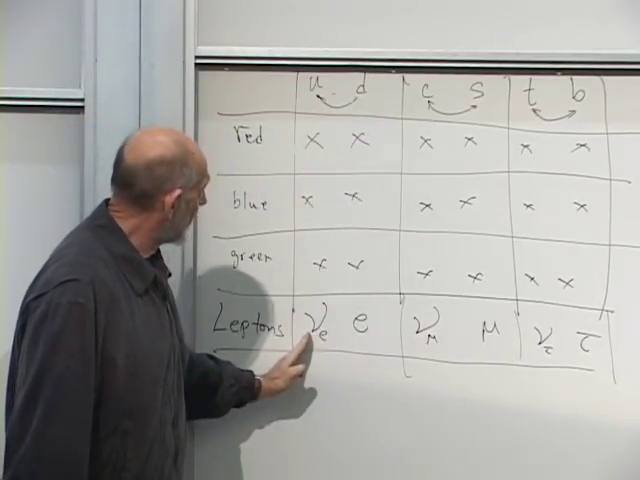
\includegraphics[width=0.82\textwidth]{lecture_05_figure_05.png}
\caption{黑板上的表格：色在红、蓝、绿行之间作用，而弱\(SU(2)\)连接成对的味列和轻子行。}
\lectureframe{01:03:35}
\end{figure}

在这个阶段，把轻子称为第四种色只是一种类比。它们在弱二重态表中占据第四行，但普通的QCD \(SU(3)\)不会把夸克旋转成轻子。

\section{构造带电弱玻色子}

\subsection{带电玻色子的量子数}

规范玻色子携带从一个二重态成员移动到另一个成员所需的变换性质。从轻子对
\(e^-\bar\nu_e\)开始。它具有电荷\(-1\)，因此相应的带电规范玻色子称为\(W^-\)：
\begin{equation}
W^-\sim e^-\bar\nu_e.
\end{equation}
相同的量子数来自下夸克和反上夸克：
\begin{equation}
W^-\sim d\bar u.
\end{equation}
符号\(\sim\)表示具有相同的相关规范量子数。它并不意味着\(W\)字面上是这些粒子的束缚态。反粒子具有共轭组合，
\begin{equation}
W^+\sim e^+\nu_e\sim\bar d u.
\end{equation}

带电弱顶点包括
\begin{align}
e^-&\longrightarrow\nu_e+W^-,
&
\mu^-&\longrightarrow\nu_\mu+W^-,
\label{eq:l5-lepton-w}\\
d&\longrightarrow u+W^-,
&
s&\longrightarrow c+W^-,
\label{eq:l5-quark-w}
\end{align}
当运动学允许时，第三代有类似的跃迁。规范玻色子动态地执行与对称性作用于二重态相同的水平混合。

\begin{classroomqa}
\audiencequestion{电荷守恒要求所发射的玻色子具有电荷\(-1\)，但为什么电子、下夸克和奇异夸克的跃迁都必须涉及同一种粒子？
\lecturetimestamp{01:12:56}}
\lecturerresponse{这是一个由共同的弱对称性所编码的经验事实。自然界本可以一致地为每个家族或分别为夸克和轻子指定不同的\(W\)型玻色子。然而，一个\(SU(2)\)同时作用于所有二重态，并且相同的带电规范玻色子媒介了所有这些跃迁。}
\end{classroomqa}

\subsection{读取和反转一个顶点}

单个顶点代表一族过程。将一条入射线反转为出射线会把粒子变成其反粒子，而反转一条\(W^-\)线则给出一个\(W^+\)。因此，只要一致地追踪电荷、动量和所有相关量子数，就可以把一个顶点读作发射、吸收、衰变、湮灭或逆反应。

\begin{classroomqa}
\audiencequestion{这些弱顶点中的箭头和线可以翻转吗？
\lecturetimestamp{01:14:51}}
\lecturerresponse{可以。一条线可以从末态跨到初态，或反之，但粒子随后变成其反粒子。因此，同一个局域顶点描述了许多取向不同的反应。}
\end{classroomqa}

\begin{classroomqa}
\audiencequestion{把一个\(W^-\)写成带有奇异线和粲线的形式，是否意味着该玻色子字面上是一个奇异夸克与一个反粲夸克束缚在一起？
\lecturetimestamp{01:15:43}}
\lecturerresponse{不是。线的记账只说明\(W^-\)携带了那些列之间的量子数变化。如果将该图读作衰变，一个能量足够高的\(W^-\)可以产生一个奇异夸克和一个反粲夸克；它并不是由它们组成的。}
\end{classroomqa}

\begin{classroomqa}
\audiencequestion{一个电子和一个反中微子能产生一个\(W\)，然后该玻色子再产生一对夸克吗？
\lecturetimestamp{01:17:22}}
\lecturerresponse{正是如此。如果有足够的质心能量，初始轻子可以形成带电流中间态，而该态可以通过允许的夸克道出现。这两个顶点与衰变中所用的是同一对顶点，只是以另一种取向来读取。}
\end{classroomqa}

\subsection{缺失的第三种玻色子}

一个\(SU(2)\)群有三个生成元，因此有三个规范场。到目前为止，我们只展示了\(W^+\)和\(W^-\)。第三个电中性场必须与诸如电子--正电子和 neutrino--antineutrino 量子数这样的对角组合相关联。它被有意留在背景中潜伏。它与物理的\(Z\)玻色子和光子之间的关系需要电弱混合，这将在后面讨论。

\begin{classroomqa}
\audiencequestion{弱力和强力是在不同的历史时期被怀疑存在的吗？
\lecturetimestamp{01:24:11}}
\lecturerresponse{它们的实验根源一起出现在早期放射性中。{\proseunicodefont α}衰变揭示了核物理和强相互作用物理，{\proseunicodefont β}衰变揭示了弱相互作用，而{\proseunicodefont γ}衰变发射电磁光子。贝克勒尔的时代就已经包含了全部三条线索，远早于它们的现代场论存在之前。}
\end{classroomqa}

\section{带电流衰变实例}

\subsection{{\proseunicodefont π}介子衰变}

带负电的{\proseunicodefont π}介子具有价夸克内容
\begin{equation}
\pi^-=d\bar u.
\end{equation}
这些量子数可以湮灭成一个\(W^-\)，后者随后可以产生一个带电轻子和相应的反中微子：
\begin{align}
\pi^-&\longrightarrow W^{-*}
\longrightarrow e^-+\bar\nu_e,
\label{eq:l5-pion-electron}\\
\pi^-&\longrightarrow W^{-*}
\longrightarrow \mu^-+\bar\nu_\mu.
\label{eq:l5-pion-muon}
\end{align}
星号提醒我们，中间的\(W\)是虚的。第二个道是主导道。

\begin{figure}[htbp]
\centering
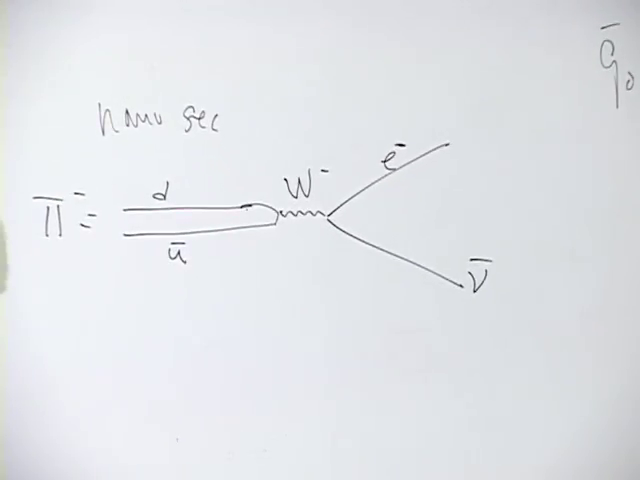
\includegraphics[width=0.72\textwidth]{lecture_05_figure_04.png}
\caption{一个\(d\bar u\){\proseunicodefont π}介子湮灭成一个虚\(W^-\)，随后产生一个带电轻子及其匹配的反中微子。}
\lectureframe{01:19:38}
\end{figure}

\begin{classroomqa}
\audiencequestion{尽管时间方向被画成水平而非垂直，这真的还是一个费曼图吗？
\lecturetimestamp{01:20:21}}
\lecturerresponse{是的。时间在纸面上的取向是一种约定。一旦声明某个方向为时间，并且所有箭头都被一致地解释，该图就携带相同的相互作用信息。}
\end{classroomqa}

\begin{classroomqa}
\audiencequestion{这个图是否可以更像一个可逆化学反应来读，而不是一个不可逆的单向衰变？
\lecturetimestamp{01:21:35}}
\lecturerresponse{逆过程是允许的。在真空中产生的{\proseunicodefont π}介子会衰变，因为出射粒子分离开来，通常不会重新结合。但是，如果一个{\proseunicodefont μ}子和反中微子以合适的能量和动量一起射入，就存在一个非零振幅通过逆相互作用形成{\proseunicodefont π}介子。}
\end{classroomqa}

\subsection{能量与虚中间态}

对于静止的{\proseunicodefont π}介子，
\begin{equation}
m_\pi\simeq140\ {\rm MeV},
\qquad
m_\mu\simeq106\ {\rm MeV},
\qquad
m_\nu\approx0
\end{equation}
在此处相关的精度下成立。剩余能量成为出射粒子的动能。动量守恒要求
\begin{equation}
\boldsymbol p_\mu+\boldsymbol p_{\bar\nu}=0,
\end{equation}
因此这两个粒子在{\proseunicodefont π}介子静止系中背对背飞出。

\begin{classroomqa}
\audiencequestion{当中间态的\(W\)远比{\proseunicodefont π}介子重时，能量如何能够守恒？
\lecturetimestamp{01:25:08}}
\lecturerresponse{只有初态和末态粒子必须处于其质量壳上。四动量在每个顶点处守恒，但内部虚线不必满足\(E^2=\boldsymbol p^2+m_W^2\)。其离壳失配越大，其传播子对该过程的压低就越强。\editorialnote{讲座使用了传统的能量--时间不确定性语言，并说中间态可以短暂地违反能量守恒。现代精确的表述是回答中的那一个：能量-动量守恒，而虚的内部线不必满足实粒子的质量壳条件。}}
\end{classroomqa}

\subsection{{\proseunicodefont μ}子衰变}

{\proseunicodefont μ}子可以先通过发射一个虚\(W^-\)而变成它自己的中微子：
\begin{equation}
\mu^-\longrightarrow\nu_\mu+W^{-*}.
\end{equation}
然后该虚玻色子产生一个电子和一个电子反中微子：
\begin{equation}
\mu^-\longrightarrow
\nu_\mu+e^-+\bar\nu_e.
\label{eq:l5-muon-decay}
\end{equation}
这是一个纯轻子过程。{\proseunicodefont μ}子比电子重约两百倍，因此末态的静止质量留下了充足的动能。

\begin{figure}[htbp]
\centering
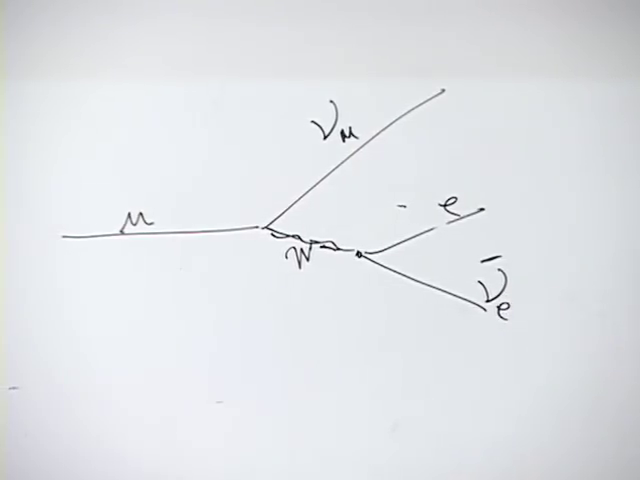
\includegraphics[width=0.72\textwidth]{lecture_05_figure_06.png}
\caption{通过虚带电弱玻色子发生的{\proseunicodefont μ}子衰变。}
\lectureframe{01:29:24}
\end{figure}

\begin{classroomqa}
\audiencequestion{与电子一起发射的中性粒子是反中微子吗？
\lecturetimestamp{01:29:06}}
\lecturerresponse{是的。完整的末态包含一个{\proseunicodefont μ}中微子、一个电子反中微子和电子。保留味标签可以防止这两个中性粒子被混淆。}
\end{classroomqa}

电子无法在真空中逆转这一衰变，因为它比{\proseunicodefont μ}子轻。{\proseunicodefont τ}子更重，可以通过类似的弱相互作用道衰变。这里的稳定性部分是质量排序的偶然结果，而不是底层顶点的差异。

\begin{classroomqa}
\audiencequestion{直线加速器是否有效地增加了电子的质量，从而使原本禁戒的反应能够反向进行？
\lecturetimestamp{01:30:23}}
\lecturerresponse{它并不改变电子的不变静止质量，而是提供动能。足够的质心能量可以产生更重的末态粒子，因此一旦把质量替换为可用的碰撞能量，所提出的物理想法就是正确的。}
\end{classroomqa}

\subsection{夸克层次上的中子{\proseunicodefont β}衰变}

中子和质子的价夸克组成为
\begin{equation}
n=udd,
\qquad
p=uud.
\end{equation}
中子中的一个下夸克发生带电流跃迁
\begin{equation}
d\longrightarrow u+W^{-*},
\end{equation}
将\(udd\)变成\(uud\)。然后该虚玻色子衰变：
\begin{equation}
W^{-*}\longrightarrow e^-+\bar\nu_e.
\end{equation}
将两个顶点结合起来就重现了
\begin{equation}
n\longrightarrow p+e^-+\bar\nu_e.
\end{equation}

相反的夸克跃迁\(u\to d+W^+\)会留下一个三下夸克重子，但那个可达到的态对于自由中子来说太重，无法产生。实际的从下到上的路径才是能量上允许的那一条。

\begin{classroomqa}
\audiencequestion{中子能否改为衰变成一个质子、一个{\proseunicodefont μ}子和相应的反中微子？
\lecturetimestamp{01:32:38}}
\lecturerresponse{对于静止的自由中子不能：中子--质子的质量差远小于{\proseunicodefont μ}子质量。如果有足够的额外碰撞能量或激发能量，同一个弱顶点可以参与产生{\proseunicodefont μ}子的道。这种禁戒是运动学的，而不是缺少相互作用。}
\end{classroomqa}

\section{未解决的压低问题}

带电弱顶点解释了哪些过程可以发生，但还没有解释它们为何如此缓慢。一个诱人的答案会是极其微小的弱耦合。这个答案是错误的：无量纲的弱规范耦合大致与电磁耦合大小相当。这种压低必定来自别的东西。

缺失的成分已经在虚传播子中显现出来：\(W\)非常重。在远低于\(m_W\)的能量下，带电流振幅大致被\(1/m_W^2\)的幂次压低。这一联系将在希格斯机制和电弱对称性破缺解释规范玻色子如何获得质量之后展开。
\editorialnote{讲座将此保留为下次会议的谜题。重\(W\)解释在此作为前瞻性联系被纳入，而不是声称其推导发生在本讲座中。}

\begin{classroomqa}
\audiencequestion{当我们说该理论具有这种对称性时，我们是指它的拉格朗日量在相应的操作下不变吗？
\lecturetimestamp{01:34:14}}
\lecturerresponse{正是如此。该理论具有对称性这一说法，是拉格朗日量——或等价地，作用量——在这些变换下不变的简写。写出完整的拉格朗日量是被推迟了，而不是被一个不同的定义所取代。}
\end{classroomqa}

这条路线现在完整了：麦克斯韦理论提供了原型；QCD 展示了非阿贝尔规范玻色子如何携带和交换荷；耦合常数解释了原子时间尺度与强子时间尺度之间的对比；而弱 \(SU(2)\) 将夸克和轻子组织成由 \(W^\pm\) 连接的二重态。剩下的任务是理解为什么这些由规范相互作用中介的过程在实践中很弱，尽管它们底层的耦合并不是特别小。